% !TeX root = ../../infdesc.tex
\hintsection{\Cref*{chGettingStarted}}

Antes de podermos começar a provar coisas, precisamos eliminar certos tipos de afirmações que poderíamos tentar provar. Considere a seguinte afirmação:

\begin{center}
\textit{Essa sentença é falsa.}
\end{center}

Isso e verdadeiro ou falso? Se você pensar sobre isso por alguns segundos, você ficará em apuros.

Agora considere a seguinte sentença :

\begin{center}
\textit{O burro mais feliz do mundo.}
\end{center}

Isso e verdadeiro ou falso? Bem, não é nem uma frase; não faz sentido nem \textit{perguntar} se é verdadeiro ou falso!

É claro que estaremos desperdiçando nosso tempo tentando escrever provas de afirmações como as duas listadas acima – precisamos restringir nosso escopo a afirmações que possamos realmente ter uma chance de provar (ou talvez refutar)! Isso motiva a seguinte definição (informal).

\begin{definition}
\label{defProposition}
\label{defProof}
\index{proposição}
\index{prova}
Uma \textbf{proposição} \index{proposição} é a declaração na qual é possível atribuir a \textbf{Valor verdadeiro} (`verdadeiro' ou `falso'). Se uma proposição é verdadeira, uma \textbf{prova} da preposição é um argumento logicamente válido que demonstra que é verdadeiro, apresentado a um nível tal que um membro do público-alvo possa verificar a sua veracidade.
\end{definition}

Assim, as afirmações dadas acima são proposições porque não há forma possível de lhes atribuir um valor de verdade. Observe que, em \Cref{defProposition}, tudo o que importa é que \textit{faz sentido} dizer que é verdadeiro ou falso, independentemente de realmente \textit{ser} verdadeiro ou falso --- o valor de verdade de muitas proposições é desconhecida, mesmo as muito simples.

\begin{exercise}
Pense em um exemplo de proposição verdadeira, de proposição falsa, de proposição cujo valor de verdade você não conhece e de uma afirmação que não é uma proposição.

\end{exercise}

Os resultados em artigos e livros didáticos de matemática podem ser chamados de \textit{proposições}, mas também podem ser chamados de \textit{teoremas}, \textit{lemas} ou \textit{corolários} dependendo do uso pretendido.
\begin{itemize}
\item Uma \textbf{proposição} é um termo abrangente que pode ser usado para qualquer resultado.
\item Um \textbf{teorema} é um resultado chave que é particularmente importante.
\item Um \textbf{lema} é um resultado que é provado com o propósito de ser usado na prova de um teorema.
\item Um \textbf{corolário} é um resultado que segue de um teorema sem muito esforço adicional.
\end{itemize}
Estas não são definições precisas e não pretendem ser --- você poderia chamar cada resultado de \textit{proposição} se quisesse --- mas usar essas palavras apropriadamente ajuda os leitores a descobrir como ler um artigo. Por exemplo, se você quiser apenas folhear um artigo e encontrar seus principais resultados, procure resultados rotulados como \textit{teoremas}.

Não adianta muito tentar provar resultados se não temos nada para provar os resultados. Com isso em mente, apresentaremos agora os \textit{conjuntos de números} e provaremos alguns resultados sobre eles no contexto de quatro tópicos, a saber: divisão de inteiros, bases numéricas, números racionais e irracionais e polinômios. Estes tópicos fornecerão contexto para o material em \Cref{ptCoreConcepts}, e servirão como uma introdução aos tópicos abordados em \Cref{ptTopics}.


Não nos aprofundaremos muito neste capítulo. Em vez disso, pense nisso como um exercício de aquecimento – uma introdução rápida e leve, com mais provas a serem fornecidas no restante do livro.

\subsection*{Conjuntos}

Fundamental para a matemática é a noção de \textit{conjunto}. Estudaremos conjuntos detalhadamente em \Cref{chSets}, mas você os encontrará em todos os capítulos do livro, então levaremos algum tempo para pensar sobre eles agora. Não trataremos conjuntos formalmente neste estágio – por enquanto, a definição a seguir será o suficiente.

\begin{definition}[a ser revisado em \Cref{defSet}]
\label{defSetsPreliminary}
\lindexmmc{in}{$\in$}
Um \textbf{conjunto} é uma coleção de objetos. Os objetos nesse conjunto são chamados \textbf{elementos} do conjunto. Se $X$ é um conjunto e $x$ é um objeto, então escrevemos $x \in X$ \inlatexnb{x \textbackslash{} in X} para denotar a afirmação que $x$ é um elemento de $X$.
\end{definition}

Os conjuntos que nos interessam em primeiro lugar são os \textit{conjuntos de números}---isto é, conjuntos cujos elementos são tipos particulares de \textit{número}. Neste nível introdutório, muitos detalhes serão temporariamente varridos para debaixo do tapete; trabalharemos com um nível de precisão apropriado ao nosso estágio atual, mas que ainda nos permita desenvolver uma quantidade razoável de intuição.

Então aqui vamos nós. Aqui está uma linha infinita:
\begin{center}
\begin{tikzpicture}
\draw[latex-latex] (-5.5, 0) -- (5.5, 0) ;
\end{tikzpicture}
\end{center}
As setas indicam que se supõe que se estenda em ambas as direções sem fim. Os pontos na linha representarão números (especificamente, \textit{números reais}, um termo enganoso que será definido em \Cref{defRealsInformal}).

Agora vamos fixar um ponto nesta linha e rotulá-lo `$0$':
\begin{center}
\begin{tikzpicture}
\draw[latex-latex] (-5.5, 0) -- (5.5, 0) ;
\draw (0, 0) -- (0, 0.1) node[above] {$0$} ;
\end{tikzpicture}
\end{center}
Este ponto pode ser considerado como uma representação do número zero; é o ponto contra o qual todos os outros números serão medidos. Os números à esquerda de $0$ na reta numérica são considerados \textit{negativos}, e os à direita são \textit{positivos}; $0$ em si não é positivo nem negativo.

Finalmente, vamos fixar uma unidade de comprimento:
\begin{center}
\begin{tikzpicture}
\draw (0, 0) -- (1, 0) ;
\foreach \x in {0,1} \draw (\x, -0.1) -- (\x, 0.1)  ;
\end{tikzpicture}
\end{center}
Esta unidade de comprimento será utilizada, entre outras coisas, para comparar até que ponto os outros números diferem de zero.
\begin{definition}
\label{defNumberLine}
Uma linha infinita acima, junto com seu ponto zero fixo e comprimento unitário fixo, constituem a (\textbf{real})\textbf{linha numérica}.
\end{definition}

Usaremos a reta numérica para construir cinco conjuntos de números de nosso interesse: o conjunto $\mathbb{N}$ de \textit{números naturais} (\Cref{defNaturalNumbersInformal}), o conjunto $\mathbb{Z}$ de \textit{inteiros} (\Cref{defIntegersInformal}), o conjunto $\mathbb{Q}$ de \textit{números racionais} (\Cref{defRationalsInformal}), o $\mathbb{R}$ de \textit{ números reais} (\Cref{defRealsInformal}), e


Cada um desses conjuntos tem um caráter diferente e é usado para propósitos diferentes, como veremos mais adiante neste capítulo e ao longo deste livro.

\subsection*{Números Naturais ($\mathbb{N}$)}

Os \textit{números naturais} são os números usados para contar---são as respostas a questões da forma `quantos'---por exemplo, tenho \textit{três} tios, \textit{três} guinéus porcos e \textit{zero} gatos.

Contar é uma habilidade que os humanos possuem há muito tempo; sabemos disso porque há evidências de pessoas que usaram marcadores há dezenas de milhares de anos. As marcas de contagem fornecem um método de contar números pequenos: começando do zero, prossiga pelos objetos que deseja contar um por um e faça uma marca para cada objeto. Quando terminar, haverá tantas marcas quantos objetos. Somos ensinados desde pequenos a contar com os dedos; este é outro exemplo de fazer marcas de registro, onde agora, em vez de fazer uma marca, levantamos um dedo.

Fazer uma marca representa um \textit{incremento} na quantidade --- isto é, adicionar um. Na nossa reta numérica, podemos representar um incremento na quantidade movendo para a direita pela unidade de comprimento. Então, a distância do zero que nos movemos, que é igual ao número de vezes que nos movemos para a direita pela unidade de comprimento, é portanto, igual ao número de objetos que estão sendo contados.

\begin{definition}
\label{defNaturalNumbersInformal}
Os \textbf{números naturais} são representados pelos pontos na reta numérica que podem ser obtidos começando em $0$ e movendo-se para a direita pela unidade de comprimento qualquer número de vezes:
\begin{center}
\begin{tikzpicture}
\draw[latex-latex] (-5.5, 0) -- (5.5, 0) ;
\foreach \x in {0,1,2,3,4,5} \draw (\x, 0) -- (\x, 0.1) node[above] {$\x$} ;
\end{tikzpicture}
\end{center}
Em termos mais familiares, eles são  \textit{os números inteiros não negativos}. Nós escrevemos $\mathbb{N}$ \inlatex{mathbb\{N\}}\lindexmmc{mathbb}{$\mathbb{A}, \mathbb{B}, \dots$} para o conjunto de todos os números naturais; assim, a notação `$n \in \mathbb{N}$' significa que $n$ é um número natural.
\end{definition}

Os números naturais possuem uma estrutura matemática muito importante e interessante, e são centrais no material em \Cref{chCombinatorics}. Uma caracterização mais precisa dos números naturais será fornecida em \Cref{secPeanosAxioms}, e uma construção matemática do conjunto de números naturais pode ser encontrada em \Cref{secZFC} (ver \Cref{cnsNaturalNumbersVonNeumann}). No centro destas caracterizações mais precisas estarão as noções de “zero” e de “adicionar um” – tal como fazer marcas de contagem.

\begin{aside} % mantenha esse note sem traduzir
Alguns autores definem os números naturais como sendo os números inteiros \textit{positivos}, excluindo assim o zero. Consideramos $0$ um número natural, pois nosso principal uso dos números naturais será para contar conjuntos finitos, e um conjunto sem nada é certamente finito! Dito isto, como acontece com qualquer definição matemática, a escolha sobre se $0 \in \mathbb{N}$ ou $0 \not \in \mathbb{N}$ é uma questão de gosto ou conveniência, e é apenas uma convenção --- não é algo que possa ser provado ou refutado.
\end{aside}

\subsection*{Bases Numéricas}

Escrever números é algo que pode parecer fácil para você agora, mas provavelmente levou vários anos quando criança para realmente entender o que estava acontecendo. Historicamente, existiram muitos sistemas diferentes para representar números simbolicamente, chamados \textit{sistemas numéricos}.\index{sistema numérico} Primeiro veio o mais primitivo de todos, os marcadores de contagem, aparecendo na Idade da Pedra e ainda sendo usados para alguns propósitos hoje. Milhares de anos e centenas de sistemas de numeração depois, existe um sistema de numeração dominante, compreendido em todo o mundo: o \textbf{sistema de numeração hindu-árabe}.\index{sistema de numeração!Hindu--árabe} Este sistema de numeração consiste em dez símbolos, chamados \textit{dígitos}. É um sistema numérico \textit{posicional}, o que significa que a posição de um símbolo em uma cadeia determina seu valor numérico.

Em inglês, os \textit{algarismos arábicos} são usados como os dez dígitos:
\[0 \quad 1 \quad 2 \quad 3 \quad 4 \quad 5 \quad 6 \quad 7 \quad 8 \quad 9 \]
O dígito mais à direita em uma cadeia está na casa das unidades e o valor de cada dígito aumenta por um fator de dez movendo-se para a esquerda. Por exemplo, quando escrevemos `$2812$', o `$2$' mais à esquerda representa o número dois mil, enquanto o último `$2$' representa o número dois.

O fato de existirem dez dígitos e de o sistema numérico ser baseado em potências de dez é um acidente biológico que corresponde ao fato de a maioria dos humanos ter dez dedos. Para muitos propósitos, isso é inconveniente. Por exemplo, dez não tem muitos divisores positivos (apenas quatro: $1$, $2$, $5$ e $10$) --- isto tem implicações para a facilidade de realizar aritmética; um sistema baseado no número doze, que possui seis divisores positivos ($1$, $2$, $3$, $4$, $6$ e $12$), pode ser mais conveniente. Outro exemplo é na computação e na eletrônica digital, onde é mais conveniente trabalhar em um sistema \textit{binário}, com apenas dois dígitos ---$0$ e $1$---que representam `off' e `on' ( ou «baixa tensão» e «alta tensão»), respetivamente; a aritmética pode então ser realizada diretamente usando sequências de \textit{portas lógicas} em um circuito elétrico.

Portanto, vale a pena ter alguma compreensão dos sistemas numéricos posicionais baseados em números diferentes de dez. A abstração matemática que fazemos leva à definição de \textit{expansão base-$b$}.

\begin{definition}
\label{defBaseBExpansionPreliminary}
\index{base-$b$ expansion}
\index{number base}
Seja $b$ um número natural maior que $1$. A \textbf{base-$b$ expansão} de um número natural $n$ é a\footnote{Essa frase é problemática, pois assume que todo número natural tem apenas uma base-$b$ expansão. Na verdade, esse fato requer prova --- veja \Cref{thmBaseBExpansion}.} cadeia $d_r d_{r-1} \dots d_0$ tal que:

\begin{enumerate}[(i)]
\item $n = d_r \cdot b^r + d_{r-1} \cdot b^{r-1} + \cdots + d_0 \cdot b^0$;
\item $0 \le d_i < b$ para cada $i$; e
\item If $n>0$ então $d_r \ne 0$---a base de expansão-$b$ de zero é $0$ em todas as bases $b$.
\end{enumerate}
Certas bases numéricas têm nomes; por exemplo, as expansões base $2$, $3$, $8$, $10$ e $16$ são chamadas respectivamente de \textit{binário}, \textit{ternário}, \textit{octal}, \textit{decimal} e \textit {hexadecimal}.
\end{definition}

Antes de olharmos um exemplo de \Cref{defBaseBExpansionPreliminary} em ação, vamos examinar a definição, que é um pouco concisa à primeira vista.
\begin{itemize}
\item Condição (i) nos diz que os dígitos na cadeia nos dizem quantos de cada potência de $b$ são somados para obter $n$. Por exemplo, quando $b=10$, os dígitos da direita para a esquerda indicam as unidades, dezenas, centenas, milhares e assim por diante.
\item Condição (ii) nos diz que os dígitos em uma expansão de base $b$ devem ser menores que $b$ --- por exemplo, os dígitos de base $4$ são $0$, $1$, $2$ e $3$. Se permitíssemos mais dígitos, então coisas bobas aconteceriam --- por exemplo, se `$\mathrm{X}$' fosse um novo dígito de base $10$ representando o número dez, então `$\mathrm{X}2$' e `$102$' seriam cadeias diferentes, ambas representando o número cento e dois.
\item Condição (iii) garante que a cadeia que representa um número positivo não tenha nenhum `$0$' inicial --- caso contrário, por exemplo, `$01423$' e `$1423$' seriam cadeias diferentes representando o mesmo número natural.
\end{itemize}

\begin{example}
Considere o número $1023$. Sua expansão decimal (base-$10$) é $1023$, já que
\[ 1023 = 1 \cdot 10^3 + 0 \cdot 10^2 + 2 \cdot 10^1 + 3 \cdot 10^0 \]
Sua expansão binária (base-$2$) é $1111111111$, já que\[ 1023 = 1 \cdot 2^9 + 1 \cdot 2^8 + 1 \cdot 2^7 + 1 \cdot 2^6 + 1 \cdot 2^5 + 1 \cdot 2^4 + 1 \cdot 2^3 + 1 \cdot 2^2 + 1 \cdot 2^1 + 1 \cdot 2^0 \]

Podemos expressar números na base $36$ usando os dez dígitos usuais de $0$ a $9$ e as vinte e seis letras de $\mathrm{A}$ a $\mathrm{Z}$; por exemplo, $\mathrm{A}$ representa $10$, $\mathrm{M}$ representa $22$ e $\mathrm{Z}$ representa $35$. A expansão de base $36$ de $1023$ é $\mathrm{SF}$, já que:
\[ 1023 = 28 \cdot 36^1 + 15 \cdot 36^0 = \mathrm{S} \cdot 36^1 + \mathrm{F} \cdot 36^0 \]
\end{example}

\begin{exercise}
Encontre as expansões binária, ternária, octal, decimal, hexadecimal e de base $36$ do número $21127$, usando as letras $\mathrm{A}$--$\mathrm{F}$ como dígitos adicionais para a expansão hexadecimal ( representando os números $10$--$15$, respectivamente) e as letras $\mathrm{A}$--$\mathrm{Z}$ como dígitos adicionais para a expansão da base $36$.
\end{exercise}

Às vezes desejamos especificar um número natural em termos de sua expansão de base $b$; temos alguma notação para isso.

\begin{notation}
Seja $b>1$. Se os números $d_0,d_1,\dots,d_r$  são dígitos base-$b$  (no sentido de \Cref{defBaseBExpansionPreliminary}), então nós escrevemos:
\[ {d_rd_{r-1} \dots d_0}_{(b)} = d_r \cdot b^r + d_{r-1} \cdot b^{r-1} + \cdots + d_0 \cdot b^0 \]
para o número natural cuja expansão de base $b$ é $d_rd_{r-1} \dots d_0$. Se não houver subscrito $(b)$ e uma base não for especificada explicitamente, a expansão será assumida como base-$10$.
\end{notation}

\begin{example}
Usando nossa nova notação,nós temos:
\[ 1023 = 1111111111_{(2)} = 1101220_{(3)} = 1777_{(8)} = 1023_{(10)} = 3\mathrm{FF}_{(16)} = \mathrm{SF}_{(36)} \]
\end{example}

\subsection*{Inteiros ($\mathbb{Z}$)}

 \textit{inteiros} podem ser usados para medir a diferença entre dois números naturais. Por exemplo, suponha que eu tenha cinco maçãs e cinco bananas. Outra pessoa, também segurando maçãs e bananas, deseja negociar. Após a nossa troca, tenho sete maçãs e apenas uma banana. Assim, tenho mais duas maçãs e quatro bananas a menos.

Como um incremento na quantidade pode ser representado movendo-se para a direita na reta numérica pela unidade de comprimento, um \textit{decremento} na quantidade pode, portanto, ser representado movendo-se para a \textit{esquerda} pela unidade de comprimento. Fazer isso dá origem aos inteiros.

\begin{definition}
\label{defIntegersInformal}
Os \textbf{inteiros} são representados pelos pontos na reta numérica que podem ser obtidos começando em $0$ e movendo-se em qualquer direção pela unidade de comprimento qualquer número de vezes:

\begin{center}
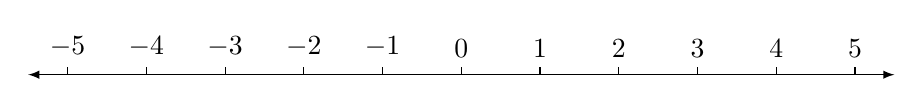
\begin{tikzpicture}
\draw[latex-latex] (-5.5, 0) -- (5.5, 0) ;
\foreach \x in {-5,-4,-3,-2,-1,0,1,2,3,4,5} \draw (\x, 0) -- (\x, 0.1) node[above] {$\x$} ;
\end{tikzpicture}
\end{center}
Nós escrevemos  $\mathbb{Z}$ \inlatex{mathbb\{Z\}}\lindexmmc{mathbb}{$\mathbb{A}, \mathbb{B}, \dots$} para o conjunto de todos os inteiros; portanto,a notação `$n \in \mathbb{Z}$' significa que $n$ é um inteiro.
\end{definition}

Os inteiros têm uma estrutura tão fascinante que um capítulo inteiro deste livro é dedicado a eles --- veja \Cref{chNumberTheory}. Isso tem a ver com o fato de que, embora seja possível somar, subtrair e multiplicar dois números inteiros e obter outro número inteiro, o mesmo não acontece com a divisão. Este “mau comportamento” da divisão é o que torna os números inteiros interessantes. Veremos agora alguns resultados básicos sobre divisão.


\subsection*{Divisão de Inteiros}
\label{pGettingStartedDivision}

A motivação que daremos em breve para a definição dos números racionais (\Cref{defRationalsInformal}) é que o resultado da divisão de um inteiro por outro inteiro não é necessariamente outro inteiro. Contudo, o resultado é \textit{às vezes} outro número inteiro; por exemplo, posso dividir seis maçãs entre três pessoas e cada pessoa receberá um número inteiro de maçãs. Isto torna a divisão interessante: como podemos medir o fracasso da divisibilidade de um número inteiro por outro? Como podemos deduzir quando um número inteiro é divisível por outro? Qual é a estrutura do conjunto de inteiros quando visto pelas lentes da divisão? Isso motiva \Cref{defDivisionPreliminary}.

\begin{definition}[Para ser repetido in \Cref{defDivision}]
\label{defDivisionPreliminary}
\index{divisão}
\index{divisor}
\index{fator}
\index{múltiplo}
Seja $a,b \in \mathbb{Z}$. Dizemos $b$ \textbf{divide} $a$ se $a=qb$ para algum inteiro $q$. Existem muitas outras maneiras de dizer que $b$ divide $a$, como: $a$ é \textit{divisível por} $b$, $b$ é um \textit{divisor} de $a$, $b $ é um \textit{fator} de $a$, ou $a$ é um \textit{múltiplo} de $b$.
\end{definition}

Observe que, talvez de forma contraintuitiva, a definição de divisibilidade não envolve a operação aritmética de divisão: ela é definida em termos de multiplicação.

\begin{example}
O inteiro $12$ é divisível por $1$, $2$, $3$, $4$, $6$ e $12$, desde que
\[ 12 = 12 \cdot 1 = 6 \cdot 2 = 4 \cdot 3 = 3 \cdot 4 = 2 \cdot 6 = 1 \cdot 12 \]
Também é divisível pelos negativos de todos esses números; por exemplo, $12$ é divisível por $-3$ desde que $12 = (-4) \cdot (-3)$.
\end{example}

\begin{exercise}
\label{exOneDividesEveryIntegerDividesZero}
Prove que $1$ divide todo número inteiro e que todo número inteiro divide $0$.
\end{exercise}

Uma consequência de \Cref{exOneDividesEveryIntegerDividesZero} é que $0$ é divisível por $0$. Isto é surpreendente: durante toda a nossa vida ouvimos que não podemos dividir por zero, mas agora descobrimos que podemos dividir zero por zero\dots{} como pode ser isso? Isso destaca por que era tão importante que a definição de divisibilidade (\Cref{defDivisionPreliminary}) fosse dada em termos de multiplicação, sem usar a operação de divisão: dizer que $0$ divide $0$ significa simplesmente que $0$ pode ser multiplicado por um inteiro para obter $0$ (o que é verdade)---mas isso não implica que a expressão `$\frac{0}{0}$' possa (ou deva) ser definida de forma significativa.

usando \Cref{defDivisionPreliminary}, podemos provar alguns fatos básicos gerais sobre a divisibilidade.


\begin{proposition}
\label{propDivisibilityIsTransitive}
Seja $a,b,c \in \mathbb{Z}$. Se $c$ divide $b$ e $b$ divide $a$, então $c$ divide $a$.
\end{proposition}

\begin{cproof}


Suponha que $c$ divide $b$ e $b$ divide $a$. Por \Cref{defDivisionPreliminary}, segue que
\[ b=qc \quad \text{e} \quad a=rb \]
para alguns inteiros $q$ e $r$. Usando a primeira equação, podemos substituir $qc$ por $b$ na segunda equação, para obter
\[ a=r(qc) \]
Mas $r(qc) = (rq)c$, e $rq$ é um número inteiro, então segue de \Cref{defDivisionPreliminary} que $c$ divide $a$.
\end{cproof}

% To do: draw attention to the wording of the proof, and the 'unpack definition - do something - apply definition' style of the proof.

\begin{exercise}
\label{exDivisibilityIsLinear}
Sejam $a,b,d \in \mathbb{Z}$. Suponha que $d$ divide $a$ e $d$ divide $b$. Dados inteiros $u$ e $v$, prove que $d$ divide $au+bv$.
\end{exercise}

Alguns conceitos familiares, como par e impar, podem ser caracterizados em termos de divisibilidade.

\begin{definition}
\label{defEvenOdd}
\index{Inteiro!par}
\index{Inteiro!´impar}
Um inteiro $n$ é \textbf{par} se é divisível por $2$; de outra forma, $n$ é \textbf{impar}.
\end{definition}
Não é apenas interessante saber quando um inteiro \textit{divide} outro; entretanto, provar que um inteiro \textit{não} divide outro é muito mais difícil. Na verdade, para provar que um inteiro $b$ não divide um inteiro $a$, devemos provar que $a \ne qb$ para \textit{qualquer} inteiro $q$. Veremos métodos para fazer isso em \Cref{chLogicalStructure}; esses métodos usam o seguinte resultado extremamente importante, que será a base de todo o \Cref{chNumberTheory}.

\begin{theorem}[Teorema da divisão, para ser repetido in \Cref{thmDivisionTheorem}]
\label{thmDivisionPreliminary}
\index{teorema da divisão}
Seja $a,b \in \mathbb{Z}$ com $b \ne 0$. Existe exatamente uma maneira de escrever
\[ a = qb + r \]
de tal modo que $q$ e $r$ são inteiros, e $0 \le r < b$ (se $b > 0$) ou $0 \le r < -b$ (se $b < 0$).
\end{theorem}

O número $q$ em \Cref{thmDivisionPreliminary} é chamado o \textbf{quociente}\index{quociente} de $a$ quando dividido por $b$, e o número $r$ é chamado o \textbf{restante}\index{restante}.

\begin{example}
O número $12$ deixa um  restante de $2$ quando dividido por $5$, desde que $12 = 2 \cdot 5 + 2$.
\end{example}

Aqui está um exemplo um pouco mais complicado.

\begin{proposition}
Suponha um número inteiro $a$ deixa um resto de $r$ quando dividido por um número inteiro $b$, e que $r>0$. Então $-a$ deixa um resto de $b-r$ quando dividido por $b$.
\end{proposition}

\begin{cproof}
Suponha que $a$ deixa um resto de $r$ quando dividido por $b$. Então
\[ a=qb+r \]
Para algum número inteiro $q$. Um pouco de álgebra nos dá
\[ -a = -qb-r = -qb-r+(b-b) = -(q+1)b + (b-r) \]
Com $0<r<b$, nós temos $0<b-r<b$. Por isso $-(q+1)$ é o quociente de $-a$ quando dividido por $b$, e $b-r$ é o restante.
\end{cproof}

\begin{exercise}
Prove que se um inteiro $a$ deixa um resto $r$ quando dividido por um inteiro $b$, então $a$ deixa um resto de $r$ quando dividido por $-b$.
\end{exercise}

Terminaremos esta parte sobre divisão de inteiros conectando-a com o material em bases numéricas --- podemos usar o teorema da divisão (\Cref{thmDivisionPreliminary}) para encontrar a expansão de base $b$ de um determinado número natural. É baseado na seguinte observação: o número natural $n$ cuja expansão de base $b$ é $d_rd_{r-1} \cdots d_1 d_0$ é igual a
\[ d_0 + b(d_1 + b(d_2 + \cdots + b(d_{r-1} + bd_r) \cdots)) \]
Além disso, $0 \le d_i < b$ para todo $i$. Em particular, $n$ deixa um resto de $d_0$ quando dividido por $b$. Por isso
\[ \frac{n-d_0}{b} = d_1 + d_2b + \cdots + d_rb^{r-1} \]
A expansão de base $b$ de $\frac{n-d_0}{b}$ é portanto
\[ d_rd_{r-1} \cdots d_1 \]
Em outras palavras, o resto de $n$ quando dividido por $b$ é o último dígito de base $b$ de $n$, e então subtrair esse número de $n$ e dividir o resultado por $b$ trunca o dígito final. Repetir esse processo nos dá $d_1$, e depois $d_2$, e assim por diante, até chegarmos a $0$.
Isso sugere o seguinte algoritmo para calcular a expansão de base $b$ de um número $n$:
\begin{itemize}
\item \textbf{Passo 1.} SeJA $d_0$ seja o resto quando $n$ é dividido por $b$, e Seja $n_0=\frac{n-d_0}{b}$ seja o quociente. Consertar $i=0$.
\item \textbf{Step 2.} Suponha $n_i$ e $d_i$ foram definidos. Se $n_i=0$, em seguida, prossiga para o Passo 3. Senão, defina $d_{i+1}$ como resto quando $n_i$ é dividido por $b$ e defina $n_{i+1} = \frac{n_i-d_{i+1}}{b}$. Incremente $i$ e repita a Etapa 2.
\item \textbf{Etapa 3.} A expansão base-$b$ de $n$ é
\[ d_id_{i-1} \cdots d_0 \]
\end{itemize}

\begin{example}
Calculamos a expansão de base $17$ de $15213$, usando as letras $\mathrm{A}$--$\mathrm{G}$ para representar os números $10$ até $16$.
\begin{itemize}
\item $15213 = 894 \cdot 17 + 15$, então $d_0=15=\mathrm{F}$ e $n_0=894$.
\item $894 = 52 \cdot 17 + 10$, então $d_1=10 = \mathrm{A}$ e $n_1=52$.
\item $52 = 3 \cdot 17 + 1$, então $d_2 = 1$ and $n_2=3$.
\item $3 = 0 \cdot 17 + 3$, então $d_3 = 3$ e $n_3=0$.
\item A expansão base -$17$ de $15213$ é portanto $31\mathrm{AF}$.
\end{itemize}
Uma rápida verificação
\[ 31\mathrm{AF}_{(17)} = 3 \cdot 17^3 + 1 \cdot 17^2 + 10 \cdot 17 + 15 = 15213 \]
como desejado.
\end{example}

\begin{exercise}
Encontre a expansão de base $ 17$ de $ 408\,735\,787$ e a expansão de base $36$ de $1\,442\,151\,747$.
\end{exercise}

\subsection*{Números Racionais ($\mathbb{Q}$)}

Cansado de comer maçã e banana, compro uma pizza dividida em oito fatias. Um amigo e eu decidimos dividir a pizza. Não tenho muito apetite, então como três fatias e meu amigo come cinco. Infelizmente, não podemos representar a proporção da pizza que cada um de nós comeu usando números naturais ou inteiros. Porém, não estamos muito longe: podemos contar o número de partes iguais em que a pizza foi dividida e, dessas partes, podemos contar quantas tivemos. Na reta numérica, isso poderia ser representado dividindo o segmento de reta unitária de $0$ a $1$ em oito partes iguais e procedendo a partir daí. Este tipo de procedimento dá origem aos \textit{números racionais}.

\begin{definition}
\label{defRationalsInformal}
Os \textbf{números racionais} são representados pelos pontos na reta numérica que podem ser obtidos dividindo qualquer um dos segmentos da reta unitária entre inteiros em um número igual de partes.
\begin{center}
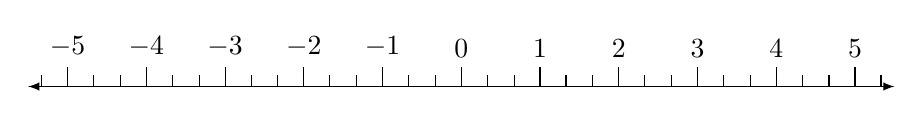
\begin{tikzpicture}
\draw[latex-latex] (-5.5, 0) -- (5.5, 0) ;
\foreach \x in {-5,-4,-3,-2,-1,0,1,2,3,4,5} \draw (\x, 0) -- (\x, 0.25) node[above] {$\x$} ;
\foreach \x in {-5,-4,-3,-2,-1,0,1,2,3,4,5} {
  \foreach \i in {-0.33,0.33} {
    \draw (\x+\i, 0) -- (\x+\i, 0.15) ;
  }
}
\end{tikzpicture}
\end{center}
Os números racionais são aqueles da forma $\frac{a}{b}$, onde $a,b \in \mathbb{Z}$ e $b \ne 0$. Escrevemos $\mathbb{Q}$ \inlatex{mathbb\{Q\}}\lindexmmc{mathbb}{$\mathbb{A}, \mathbb{B}, \dots$} para o conjunto de todos os números racionais; portanto, a notação `$q \in \mathbb{Q}$' significa que $q$ é um número racional.\end{definition}

Os números racionais são um exemplo muito importante de um tipo de estrutura algébrica conhecida como \textit{campo} --- eles são particularmente centrais para a teoria algébrica dos números e para a geometria algébrica.

\subsection*{Números reais ($\mathbb{R}$)}

Quantidade e mudança podem ser medidas de forma abstrata usando \textit{números reais}.

\begin{definition}
\label{defRealsInformal}
Os \textbf{números reais} são os pontos na reta numérica. Escrevemos $\mathbb{R}$ \inlatex{mathbb\{R\}}\lindexmmc{mathbb}{$\mathbb{A}, \mathbb{B}, \dots$} para o conjunto de todos os números reais; portanto, a notação `$a \in \mathbb{R}$' significa que $a$ é um número real.

\end{definition}

Os números reais são centrais para a análise real, um ramo da matemática introduzido em \Cref{chRealNumbers}. Eles transformam os racionais em um \textit{continuo} ao `preencher as lacunas'---especificamente, eles têm a propriedade de \textit{completude}, o que significa que se uma quantidade pode ser aproximada com precisão arbitrária por números reais, então essa quantidade é em si um número real.

Podemos definir as operações aritméticas básicas (adição, subtração, multiplicação e divisão) sobre os números reais, e uma noção de ordenação dos números reais, em termos da reta numérica infinita.
\begin{itemize}
\item \textbf{Ordenando.} Um número real $a$ é menor que um número real $b$, escrito $a<b$, se $a$ estiver à esquerda de $b$ na reta numérica. As convenções usuais para os símbolos $\le$ \inlatex{le}\lindexmmc{le}{$\le$}, $>$ e $\ge$ \inlatex{ge}\lindexmmc{ge}{$\ge$ } se aplicam, por exemplo `$a \le b$' significa que $a < b$ ou $a = b$.

\item \textbf{Adição.} Suponha que queiramos adicionar um número real $a$ a um número real $b$. Para fazer isso, \textit{traduzimos} $a$ em $b$ unidades para a direita --- se $b<0$ então isso equivale a traduzir $a$ em um número equivalente de unidades para a esquerda. Concretamente, faça duas cópias da reta numérica, uma acima da outra, com a mesma escolha de comprimento unitário; mova o $0$ da reta numérica inferior abaixo do ponto $a$ da reta numérica superior. Então $a+b$ é o ponto na reta numérica superior situado acima do ponto $b$ da reta numérica inferior.
 $(-3) + 5 = 2$:

\begin{center}
\fitwidthc{0.9}{\begin{tikzpicture}
% Adapted from http://tex.stackexchange.com/questions/148252/
\draw[latex-latex] (-8.5,0) -- (5.5,0) ;
\foreach \x in  {-8,-7,-6,-5,-4,-3,-2,-1,0,1,2,3,4,5}
\draw[shift={(\x,0)}] (0pt,3pt) -- (0pt,-3pt);
\foreach \x in {-8,-7,-6,-5,-4,-3,-2,-1,0,1,2,3,4,5}
\draw[shift={(\x,0)}] (0pt,0pt) -- (0pt,3pt) node[above] {$\x$};
\draw[*-*] (-3.08,0) -- (2.08,0);
\draw[very thick] (-3,0) -- (2,0);

\draw[latex-latex] (-8.5,-1) -- (5.5,-1) ;
\foreach \x in  {-5,-4,-3,-2,-1,0,1,2,3,4,5,6,7,8}
\draw[shift={(\x-3,-1)},color=black] (0pt,3pt) -- (0pt,-3pt);
\foreach \x in {-5,-4,-3,-2,-1,0,1,2,3,4,5,6,7,8}
\draw[shift={(\x-3,-1)},color=black] (0pt,0pt) -- (0pt,-3pt) node[below] {$\x$};
\draw[dashed] (-3,-1) -- (-3,0) ;
\draw[->] (2,-0.8) -- (2,-0.2) ;
\end{tikzpicture}}
\end{center}

\item \textbf{Multiplicação.} Este é divertido. Suponha que queiramos multiplicar um número real $a$ por um número real $b$. Para fazer isso, \textit{escala} a reta numérica e talvez a \textit{reflete}. Concretamente, faça duas cópias da reta numérica, uma acima da outra; alinhe os pontos $0$ em ambas as retas numéricas e estique a reta numérica inferior uniformemente até que o ponto $1$ na reta numérica inferior esteja abaixo do ponto $a$ na reta numérica superior --- observe que se $a<0$ então a reta numérica deve ser refletida para que isso aconteça. Então $a \cdot b$ é o ponto na reta numérica superior situado acima de $b$ na reta numérica inferior.
 $5 \cdot 4 = 20$.

\begin{center}
\fitwidthc{0.9}{\begin{tikzpicture}
% Adapted from http://tex.stackexchange.com/questions/148252/
\draw[latex-latex] (-5.5,0) -- (8.5,0) ;
\foreach \x in  {-2,-1,0,1,2,3,4,5,6,7,8,9,10,11,12,13,14,15,16,17,18,19,20,21,22,23,24}
\draw[shift={(0.5*\x-4,0)}] (0pt,3pt) -- (0pt,-3pt);
\foreach \x in {-2,-1,0,1,2,3,4,5,6,7,8,9,10,11,12,13,14,15,16,17,18,19,20,21,22,23,24}
\draw[shift={(0.5*\x-4,0)}] (0pt,0pt) -- (0pt,3pt) node[above] {$\text{\footnotesize\x}$};
\draw[*-*] (-1.58,0) -- (6.08,0);
\draw[very thick] (-1.5,0) -- (6,0);

\draw[latex-latex] (-5.5,-1) -- (8.5,-1) ;
\foreach \x in  {0,1,2,3,4}
\draw[shift={(2.5*\x-4,-1)},color=black] (0pt,3pt) -- (0pt,-3pt);
\foreach \x in {0,1,2,3,4}
\draw[shift={(2.5*\x-4,-1)},color=black] (0pt,0pt) -- (0pt,-3pt) node[below] {$\x$};
\draw[dashed] (-4,-1) -- (-4,0) ;
\draw[dashed] (-1.5,-1) -- (-1.5,0) ;
\draw[->] (6,-0.8) -- (6,-0.2) ;
\end{tikzpicture}}
\end{center}

e aqui está uma ilustração do fato de que $(-5) \cdot 4 = -20$:
\begin{center}
\fitwidthc{0.9}{\begin{tikzpicture}
% Adapted from http://tex.stackexchange.com/questions/148252/
\draw[latex-latex] (-5.5,0) -- (8.5,0) ;
\foreach \x in  {-22,-21,...,4}
\draw[shift={(0.5*\x+6,0)}] (0pt,3pt) -- (0pt,-3pt);
\foreach \x in {-22,-21,...,4}
\draw[shift={(0.5*\x+6,0)}] (0pt,0pt) -- (0pt,3pt) node[above] {$\text{\footnotesize\x}$};
\draw[*-*] (-4.08,0) -- (3.58,0);
\draw[very thick] (-4,0) -- (3.5,0);

\draw[latex-latex] (-5.5,-1) -- (8.5,-1) ;
\foreach \x in  {0,1,2,3,4}
\draw[shift={(6-2.5*\x,-1)},color=black] (0pt,3pt) -- (0pt,-3pt);
\foreach \x in {0,1,2,3,4}
\draw[shift={(6-2.5*\x,-1)},color=black] (0pt,0pt) -- (0pt,-3pt) node[below] {$\x$};
\draw[dashed] (6,-1) -- (6,0) ;
\draw[dashed] (3.5,-1) -- (3.5,0) ;
\draw[->] (-4,-0.8) -- (-4,-0.2) ;
\end{tikzpicture}}
\end{center}
\end{itemize}

\begin{exercise}
Interprete as operações de subtração e divisão como transformações geométricas da reta numérica real.\end{exercise}

Tomaremos como certas as propriedades aritméticas dos números reais neste capítulo, esperando até \Cref{secInequalitiesMeans} para nos aprofundamos nos detalhes. Por exemplo, tomaremos como certas as propriedades básicas dos números racionais, por exemplo
\[ \frac{a}{b}+\frac{c}{d} = \frac{ad+bc}{bd} \quad \text{and} \quad \frac{a}{b} \cdot \frac{c}{d} = \frac{ac}{bd} \]

\subsection*{Números Racionais e Irracionais}
\label{pGettingStartedRationalNumbers}

Antes de podermos falar sobre números irracionais, devemos dizer o que são.

\begin{definition}
\label{defIrrationalNumber}
\index{numéro irracional}
Um \textbf{Número irracional} é um número que não é racional.
\end{definition}

Ao contrário de $\mathbb{N},\mathbb{Z},\mathbb{Q},\mathbb{R},\mathbb{C}$, não existe uma única letra padrão que expresse os números irracionais. No entanto, até ao final de \Cref{secSetOperations}, seremos capazes de escrever o conjunto de números irracionais como `$\mathbb{R} \setminus \mathbb{Q}$'.

Provar que um número real é \textit{irracional} não é particularmente fácil, em geral. Por hora vamos assumir o seguinte resultado, que é reafirmado e provado em \Cref{propSqrt2Irrational}.

\begin{proposition}
\label{propSqrt2IrrationalPreliminary}
O número real $\sqrt{2}$ é irracional. \qed
\end{proposition}

% To do: include proof, note that we will prove that fractions can be cancelled to lowest terms later.

Podemos usar o fato de que $\sqrt{2}$ é irracional para provar alguns fatos sobre a relação entre números racionais e números irracionais.

\begin{proposition}
Sejam $a$ e $b$ números irracionais. É possível que $ab$ seja racional.
\end{proposition}

\begin{cproof}
Seja $a=b=\sqrt{2}$. Então $a$ e $b$ são irracionais,e $ab=2=\frac{2}{1}$, o que é racional.
\end{cproof}

\begin{exercise}
Seja $r$ um número racional e $a$ um número irracional. Prove que é possível que $ra$ seja racional, e é possível que $ra$ seja irracional.\end{exercise}

% To do: set-builder notation and intervals

\subsection*{Números Complexos ($\mathbb{C}$)}

Vimos que a multiplicação por números reais corresponde ao escalonamento e reflexão da reta numérica – escalonamento sozinho quando o multiplicando é positivo, e escalonamento com reflexão quando é negativo. Poderíamos alternativamente interpretar esta reflexão como uma \textit{rotação} de meia volta, uma vez que o efeito na reta numérica é o mesmo. Você pode então se perguntar o que acontece se girarmos em ângulos arbitrários, em vez de apenas meias voltas.

O que obtemos é um \textit{plano} de números, não apenas uma linha --- veja \Cref{figComplexNumbers}. Além disso, acontece que as regras que esperamos que as operações aritméticas satisfaçam ainda são válidas – a adição corresponde à translação e a multiplicação corresponde à escala e à rotação. Este conjunto de números resultante é o dos \textit{números complexos}.

\begin{definition}
\label{defComplexNumbersInformal}
Os \textbf{números complexos} são aqueles obtidos pelos números reais não negativos após rotação de qualquer ângulo em torno do ponto $0$. Escrevemos $\mathbb{C}$ \inlatex{mathbb\{C\}}\lindexmmc{mathbb}{$\mathbb{A}, \mathbb{B}, \dots$} para o conjunto de todos os números complexos; portanto, a notação `$z \in \mathbb{C}$' significa que $z$ é um número complexo.
\end{definition}

\begin{figure}[p!]
\centering
\resizebox{\textwidth}{!}{
\begin{tikzpicture}
\draw[latex-latex] (-5.5,0) -- (5.5,0) ;
\draw[latex-latex, dotted] (-4.76, 2.75) -- (4.76, -2.75) ;
\draw[latex-latex, dotted] (-2.75, 4.76) -- (2.75, -4.76) ;
\draw[latex-latex, dotted] (0, -5.5) -- (0, 5.5) ;
\draw[latex-latex, dotted] (2.75, 4.76) -- (-2.75, -4.76) ;
\draw[latex-latex, dotted] (4.76, 2.75) -- (-4.76, -2.75) ;
\draw[dotted] (0,0) circle [radius=1] ;
\draw[dotted] (0,0) circle [radius=2] ;
\draw[dotted] (0,0) circle [radius=3] ;
\draw[dotted] (0,0) circle [radius=4] ;
\draw[dotted] (0,0) circle [radius=5] ;
\foreach \x in  {-5,-4,-3,-2,-1,0,1,2,3,4,5}
  \draw[shift={(\x,0)}] (0pt,3pt) -- (0pt,-3pt);
\foreach \x in {-5,-4,-3,-2,-1,0,1,2,3,4,5}
  \draw[shift={(\x,0)}] (0,0) node[below right] {$\text{\small\x}$};
\draw (0,1) node[above right] {$i$};
\draw (-3pt,1) -- (3pt,1);
\foreach \x in {2,3,4,5}
  \draw[shift={(0,\x)}] (0,0) node[above right] {$\x i$};
\foreach \x in {2,3,4,5}
  \draw[shift={(0,\x)}] (-3pt,0pt) -- (3pt, 0pt);
\foreach \x in {2,3,4,5}
  \draw[shift={(0,-\x)}] (0,0) node[below right] {$\text{\small-}\x i$};
\foreach \x in {2,3,4,5}
  \draw[shift={(0,-\x)}] (-3pt,0pt) -- (3pt, 0pt);
\draw (0,-1) node[below right] {$\text{\small-}i$};
\draw (-3pt,-1) -- (3pt,-1);
\end{tikzpicture}
}
\caption{Ilustração do plano complexo, com alguns pontos rotulados.}
\label{figComplexNumbers}
\end{figure}

Existe um número complexo particularmente importante, $i$, que é o ponto no plano complexo exatamente uma unidade acima de $0$ --- isso é ilustrado em \Cref{figComplexNumbers}. A multiplicação por $i$ tem o efeito de girar o plano um quarto de volta no sentido anti-horário. Em particular, temos $i^2 = i \cdot i = -1$; os números complexos têm a surpreendente propriedade de que existem raízes quadradas de \textit{todos} os números complexos (incluindo todos os números reais).

Na verdade, todo número complexo pode ser escrito na forma $a+bi$, onde $a,b \in \mathbb{R}$; este número corresponde ao ponto no plano complexo obtido movendo $a$ unidades para a direita e $b$ unidades para cima, invertendo as direções como de costume se $a$ ou $b$ for negativo. A aritmética nos números complexos funciona da mesma forma que nos números reais; em particular, usando o fato de que $i^2=-1$, obtemos
\[ (a+bi)+(c+di) = (a+c)+(b+d)i \quad \text{and} \quad (a+bi) \cdot (c+di) = (ac-bd) + (ad+bc)i \]

Discutiremos números complexos mais detalhadamente na parte deste capítulo sobre polinômios abaixo.

\subsection*{Polinômios}
\label{pGettingStartedPolynomials}

Os números naturais, inteiros, números racionais, números reais e números complexos são todos exemplos de \textit{semirings}, o que significa que eles vêm equipados com noções de adição e multiplicação bem comportadas.

\begin{definition}
\label{defPolynomialPreliminary}
\index{polinômios}
Seja $\mathbb{S} = \mathbb{N}$, $\mathbb{Z}$, $\mathbb{Q}$, $\mathbb{R}$ ou $\mathbb{C}$. Um (\textbf{univariado}) \textbf{polinômio sobre $\mathbb{S}$} no \textbf{indeterminado} $x$ é uma expressão da forma
\[ a_0 + a_1x + \cdots + a_nx^n \]
onde $n \in \mathbb{N}$ e cada $a_k \in \mathbb{S}$. Os números $a_k$ são chamados de \textbf{coeficientes} do polinômio. Se nem todos os coeficientes forem zero, o maior valor de $k$ para o qual $a_k \ne 0$ é chamado de \textbf{grau} do polinômio. Por convenção, o grau do polinômio $0$ é $-\infty$.
\end{definition}

Polinômios de grau $1$, $2$, $3$, $4$ e $5$ são respectivamente chamados \textit{lineares}, \textit{quadratic}, \textit{cubic}, \textit{quartic} and \textit{quintic} polynomials.

\begin{example}
As seguintes expressões são todas polinômios:
\[ 3 \qquad 2x-1 \qquad (3+i)x^2-x \]
Seus graus são $0$, $1$ e $2$, respectivamente. Os dois primeiros são polinômios sobre $\mathbb{Z}$, e o terceiro é um polinômio sobre $\mathbb{C}$.
\end{example}

\begin{exercise}
Escreva um polinômio de grau $4$ sobre $\mathbb{R}$ que não seja um polinômio sobre $\mathbb{Q}$.
\end{exercise}

\begin{notation}
Em vez de escrever os coeficientes de um polinômio todas as vezes, podemos escrever algo como $p(x)$ ou $q(x)$. O `$(x)$' indica que $x$ é o indeterminado do polinômio. Se $\alpha$ for um número\footnote{Ao lidar com polinômios, normalmente reservaremos a letra $x$ para a variável indeterminada e usaremos as letras gregas $\alpha,\beta,\gamma$ \inlatex{alpha, \textbackslash{}beta, \textbackslash{}gamma} para números a serem substituídos em um polinômio.} e $p(x)$ é um polinômio em $x$ indeterminado, escrevemos $p(\alpha)$ para o resultado de \textbf{substituir} $\alpha$ por $x$ na expressão $p(x)$.
\end{notation}

Note que, se $A$ é qualquer um dos conjuntos $\mathbb{N}$, $\mathbb{Z}$, $\mathbb{Q}$, $\mathbb{R}$ ou $\mathbb{C}$, e $p(x)$ é um polinômio sobre $A$, então $p(\alpha) \in A$ para toda $\alpha \in A$.

\begin{example}
Seja $p(x)=x^3-3x^2+3x-1$. então $p(x)$ é um polinômio sobre $\mathbb{Z}$ com indeterminado $x$. Para qualquer número inteiro $\alpha$, o valor $p(\alpha)$ também será um número inteiro. Por exemplo
\[ p(0) = 0^3-3 \cdot 0^2 + 3 \cdot 0 - 1 = -1 \quad \text{and} \quad p(3) = 3^3 - 3 \cdot 3^2 + 3 \cdot 3 - 1 = 8 \]
\end{example}

\begin{definition}
\label{defRootOfPolynomial}
\index{raiz}
Seja $p(x)$ m polinômio. Uma \textbf{raiz} de $p(x)$ é um número complexo $\alpha$ de tal modo que $p(\alpha)=0$.
\end{definition}

A \textit{fórmula quadrática} (\Cref{thmQuadraticFormula}) nos diz que as raízes do polinômio $x^2+ax+b$, onde $a,b \in \mathbb{C}$, são precisamente os números complexos
\[ \frac{-a+\sqrt{a^2-4b}}{2} \quad \text{e} \quad \frac{-a-\sqrt{a^2-4b}}{2} \]

Observe que evitamos o símbolo `$\pm$', que é comumente encontrado em discussões sobre polinômios quadráticos. O símbolo `$\pm$' é perigoso porque pode suprimir a palavra `e' ou a palavra `ou', dependendo do contexto --- este tipo de ambigüidade não é algo com o qual desejaremos lidar ao discutir a estrutura lógica de uma proposição em \Cref{chLogicalStructure}!

\begin{example}
\label{exApplicationOfQuadraticFormula}
Seja $p(x)=x^2-2x+5$. A fórmula quadrática nos diz que as raízes de $p$ são
\begin{center}
$\dfrac{2 + \sqrt{4 - 4 \cdot 5}}{2} = 1 + \sqrt{-4} = 1+2i$
\quad and \quad
$\dfrac{2 - \sqrt{4 - 4 \cdot 5}}{2} = 1-\sqrt{-4} = 1-2i$
\end{center}
Os números $1+2i$ e $1-2i$ estão relacionados porque suas partes reais são iguais e suas partes imaginárias diferem apenas por um sinal. \Cref{exComplexNumberAsRootOfQuadraticOverR} generaliza esta observação.
\end{example}

\begin{exercise}
\label{exComplexNumberAsRootOfQuadraticOverR}
Seja $\alpha = a+bi$ um número complexo, onde $a,b \in \mathbb{R}$. Prove que $\alpha$ é a raiz de um polinômio quadrático sobre $\mathbb{R}$ e encontre a outra raiz desse polinômio.
\end{exercise}

O exercício a seguir prova o conhecido resultado que classifica o número de raízes reais de um polinômio sobre $\mathbb{R}$ em termos de seus coeficientes.

\begin{exercise}
\label{exDiscriminantRealRoots}
\index{discriminante}
Seja $a,b \in \mathbb{C}$ e seja $p(x)=x^2+ax+b$. O valor $\Delta=a^2-4b$ é chamado de \textbf{discriminante} de $p$. Prove que $p$ tem duas raízes se $\Delta \ne 0$ e uma raiz se $\Delta = 0$. Além disso, se $a,b \in \mathbb{R}$, prove que $p$ não tem raízes reais se $\Delta < 0$, uma raiz real se $\Delta = 0$, e duas raízes reais se $ \Delta > 0$.
\end{exercise}

\begin{example}
Considere o polinômio $x^2-2x+5$. Seu discriminante é igual a $(-2)^2-4 \cdot 5 = -16$, que é negativo. \Cref{exDiscriminantRealRoots} nos diz que tem duas raízes, nenhuma das quais é real. Isto foi verificado por \Cref{exApplicationOfQuadraticFormula}, onde descobrimos que as raízes de $x^2-2x+5$ are $1+2i$ e $1-2i$.

Agora considere o polinômio $x^2-2x-3$. Seu discriminante é igual a $(-2)^2-4\cdot(-3) = 16$, o que é positivo. \Cref{exDiscriminantRealRoots} nos diz que tem duas raízes, ambas reais; e realmente
\[ x^2-2x-3 = (x+1)(x-3) \]
então as raízes de $x^2-2x-3$ são $-1$ e $3$.
\end{example}
